\title{B-365 HW 2}
\author{
        Lucas Klein\\
                luklein\\
}
\date{\today}
\documentclass[12pt]{article}
\usepackage{graphicx}

\begin{document}
\maketitle

\section*{Problem 1}
100,020 Massachusetts adults were randomly sampled with two factors recorded:  whether or not the individualhad diabetes, and whether or not the person ate Kale.  The following gives a table of the results.
\begin{center}
	\begin{tabular}{c c c} 
		\hline
		\space & Diabetes & No Diabetes \\ 
		\hline
		Kale& 801 & 9192 \\ 
		\hline
		No Kale & 9905 & 80122 \\ 
		\hline
	\end{tabular}
\end{center}
\begin{center}
probability table\\
\begin{tabular}{c c c} 
	\hline
	\space & Diabetes & No Diabetes \\ 
	\hline
	Kale& 0.008 & 0.092 \\ 
	\hline
	No Kale & 0.10 & 0.801 \\ 
	\hline
\end{tabular}
\end{center}
\subsection*{(A)}

\paragraph{Answer}
p(A $\mid$ B) cannot be computed because the sample would need to be the entire population of adults in Massachusetts.

\subsection*{(B)}

\paragraph{Answer}
$\hat{p}(A \mid B)$ = P(Diabetes Kale)/Diabetes  = 0.074

\subsection*{(C)}

\paragraph{Answer}
Use the root n rule.\\
Kale\\
$\hat{p}= 0.087$
$\hat{p} +- 1.96(\sqrt{\hat{p}*(1-\hat{p})})/\sqrt{n}$\\
95\% interval = (0.07351 , 0.07449)\\
No Kale\\
$\hat{p} = 0.123$
95\% interval = (0.1209 , 0.1250)\\
\subsection*{(D)}

\paragraph{Answer}
According to the 95\% confidence intervals we should be able to conclude that kale eaters are less likely to have diabetes. The difference between the probability of having diabetes between the two groups in much greater than the size of the confidence intervals and since they do not overlap we can conclude that kale eaters are less likely to have diabetes. 

\subsection*{(E)}

\paragraph{Answer}
No, the sample left out valuable data such as age, gender, weight and other dietary questions.

\subsection*{(F)}

\paragraph{Answer}
It is possible that a lower rate of diabetes exists for kale eaters because in general people who consume kale also eat healthier in general and exercise more.

\section*{Problem 2}
Consider the same numerical data, but imagine that the people were assigned to eat kale for 10 years, according to the following mechanisms.  In each case say if you believe there is evidence that Kale causes a lower rate of diabetes and explain why.

\subsection*{(A)}

\paragraph{Answer}
I believe their is enough evidence here to draw that conclusions as the selection is based on something not related to kale consumption or health and evenly distributed. 

\subsection*{(B)}

\paragraph{Answer}
The sample groups are selected based on health criteria which could sway the results. Therefor I do not think there would be enough evidence to make this conclusion.

\subsection*{(C)}

\paragraph{Answer}
A good conclusion could be drawn from this even though one of the groups is much smaller. This just means the 95\% confidence intervals have a great chance of overlapping and making the study inconclusive.

\section*{Problem 3}
 Consider the following computer experiment.  Generate two “uniformly distributed” numbers x, y in the interval[0,1] (this is what run if does). Let A be the event that $x+y < 1$ and B be the event that $x-y < 0$.

\subsection*{(A)}

\paragraph{Answer}
\begin{center}
	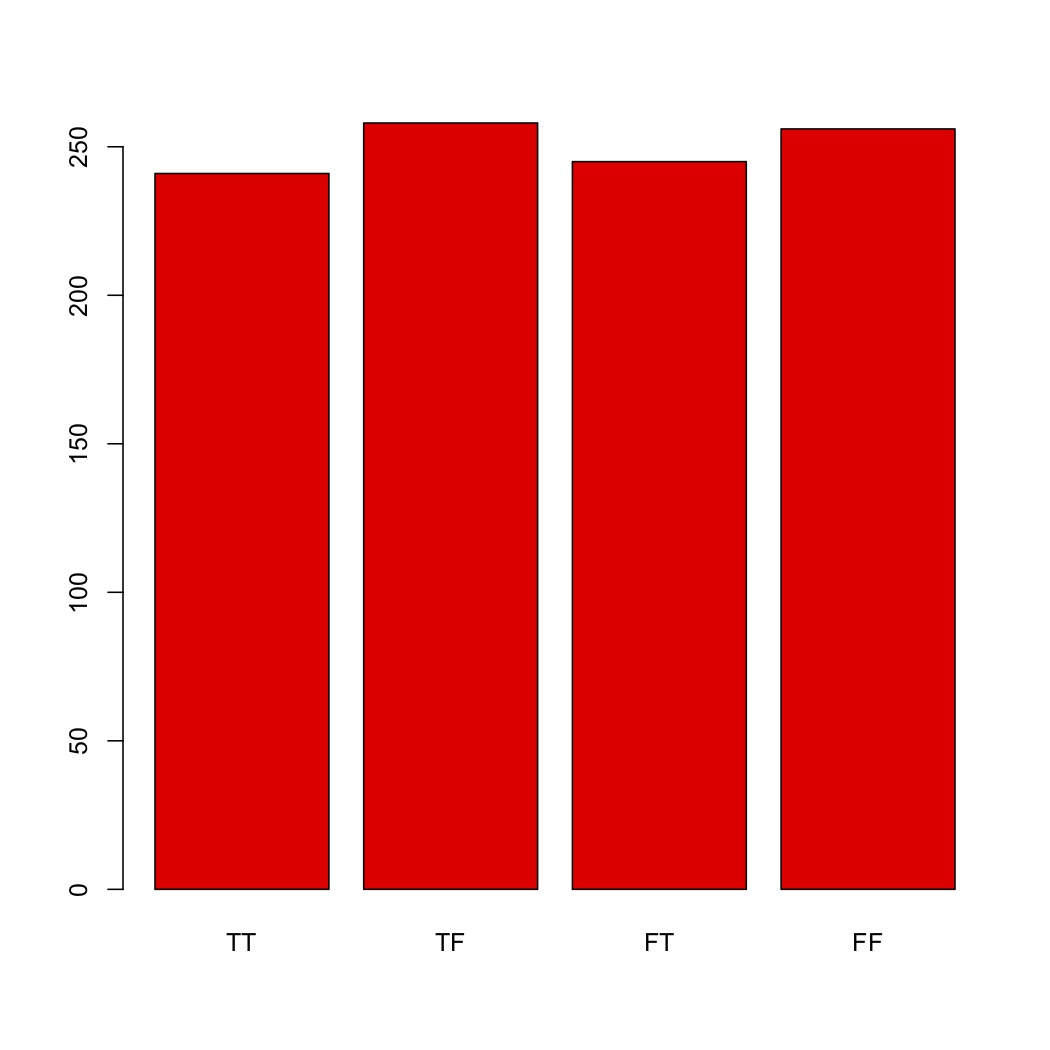
\includegraphics[width=\linewidth]{problem3Achart.jpg}
\end{center}
A and B are independent because each event is not effected by the outcome of the other event. This can be illustrated in the graph, and also if these number are put into a four way table.

\subsection*{(B)}

\paragraph{Answer}
P(A)\\
the probability is  0.5 \\
The 95\% interval is from  0.4690097 to 0.5309903\\
the half width of the interval is  0.03099032 \\
P(A and B)\\
the probability is  0.251 \\
The 95\% interval is from  0.2241259 to 0.2778741\\
the half width of the interval is  0.02687409\\
Since there is an equal chance of A happening as their is B it makes sense that if they are independent events the probability of them both happening should be the product of their probabilities. 

\section*{Problem 4}
Consider the following experiment for generating two boolean variables corresponding to the events A, B.  Here x\%\%y is the remainder when x is divided by y, so x\%\%1 is the “decimal part” of x.

\subsection*{(A)}

\paragraph{Answer}

\end{document}
This is never printed